\documentclass[preprint,12pt]{elsarticle}
\usepackage{amsmath,amssymb,bm}
\usepackage{booktabs,multirow,threeparttable}
\usepackage{graphicx,subcaption}
\usepackage{siunitx}
\usepackage{xcolor}
\usepackage{hyperref}
\usepackage{lineno}
\usepackage{enumitem}
\usepackage{microtype}
\emergencystretch=2em
\graphicspath{{../figures/}}
\hypersetup{colorlinks=true,linkcolor=blue!50!black,citecolor=blue!50!black,urlcolor=blue!60!black}
\journal{Transportation Research Part C}
\newcommand{\CNY}{\mathrm{RMB}}
\newcommand{\IJS}{\mathrm{IJS}}
\newcommand{\JS}{\mathrm{JS}}

\begin{document}
\begin{frontmatter}

\title{Data-driven collaborative optimization of three-dimensional highway alignments for life-cycle cost and mixed fuel--electric traffic energy}

\author[aff1]{Anonymous Author(s)}
\affiliation[aff1]{organization={Anonymous institution for double-anonymized review},
  city={Anonymous}, country={China}}

\begin{abstract}
Highway alignment design couples horizontal geometry, vertical profile, terrain, structures, urban development and long-term vehicle operation. Existing optimization studies often simplify one or more of these couplings, which can produce geometrically feasible but physically or economically implausible alternatives. This study develops a data-driven bi-objective framework for collaborative horizontal--vertical alignment optimization. A quasi-natural digital elevation model (DEM), OpenStreetMap (OSM) roads, railways, watercourses and building-density tiers, and 14,018 measured GNSS points are integrated in a common corridor model. The decision vector contains 50 low-frequency horizontal sine modes and 225 vertical-profile variables. Life-cycle cost covers land, basic works, bridges, tunnels, earthwork and maintenance; traffic energy monetizes 30-year fuel and electricity use for a mixed fleet. OSM intersections endogenously trigger crossing bridges, a connected high-elevation zone triggers an ecological tunnel, and dense built-up cores are treated as hard exclusions. An improved Jellyfish Search (IJS) combines independent Tent-map initialization, domain-scaled L\'evy flights and differential-evolution refinement. Entropy weighting is used to screen feasible non-dominated alternatives rather than to conceal constraint violations.

The framework is evaluated on a 22.46-km section of Guangzhou North Ring Expressway. Under the current endpoint-anchored, $\pm500$-m corridor and density-constrained setting, the selected alignment reduces life-cycle cost from 2.6406 to 2.4208 billion RMB (8.33\%) and monetized traffic energy from 1.3946 to 1.3528 billion RMB (3.00\%). The minimum horizontal radius is 421 m, the hard-constraint penalty is zero, Tier-2 exposure is zero, and Tier-1 exposure decreases from approximately 2.00 to 1.59 km. A controlled pre-density experiment further shows that sequential horizontal-then-vertical optimization attains deceptively lower objectives while violating the 400-m radius limit, whereas collaborative optimization is feasible. In a 30-run ablation, IJS improves the mean scalar objective by 25.45\% over the original Jellyfish Search; differential evolution provides the dominant contribution. Across six joint problem scales (95--500 dimensions), IJS ranks first against JS, NSGA-II, GA, PSO and GWO, with pairwise Wilcoxon tests below $8.8\times10^{-4}$. A 237-point re-optimization sensitivity experiment remains fully feasible. The results show that adding DEM/OSM constraints and enforcing horizontal--vertical coupling changes not only optimization quality but also the physical meaning of the solution.
\end{abstract}

\begin{keyword}
highway alignment optimization \sep digital elevation model \sep OpenStreetMap \sep improved Jellyfish Search \sep life-cycle cost \sep mixed traffic energy \sep horizontal--vertical coordination
\end{keyword}
\end{frontmatter}

\linenumbers

\section{Introduction}

Highway alignment is an early design decision with long-lived consequences. A small lateral shift changes the terrain crossed, land take, bridge and tunnel demand, earthwork balance, maintenance exposure and the grades experienced by vehicles. These effects are coupled: shortening a horizontal path may worsen the vertical profile; avoiding a mountain may enter a dense urban zone; lowering earthwork can require a bridge; and a profile that appears energy-efficient in one direction can become infeasible at its network tie-ins. The practical problem is therefore not a curve-fitting exercise but a constrained, spatially explicit, multi-objective design problem.

Classical formulations established the value of simultaneous horizontal and vertical optimization \cite{chew1989,jong2003}. Subsequent research introduced corridor models, mixed-integer formulations, environmental objectives and preference-aware multi-objective search \cite{kang2012,mondal2015,hirpa2016,vazquez2018,akhmet2022}. Recent work has coupled alignment generation with BIM, GIS, deep reinforcement learning and sampling-based planning \cite{han2023,he2023,alhadad2024,pu2024}. A comprehensive review by Song et al. \cite{songreview2023} nevertheless identifies enduring gaps between algorithmic models and the heterogeneous spatial constraints encountered in engineering design.

Three gaps motivate this study. First, many models use a single centerline terrain profile or stylized land-cost grid. This prevents horizontal displacement from changing the terrain and can erase the main economic reason for joint optimization. Second, bridges, tunnels and urban avoidance are commonly imposed as fixed lengths or discontinuous penalties. Such simplifications allow an optimizer to exploit bookkeeping rules rather than discover an engineering alternative. Third, large nonlinear decision spaces remain difficult for population-based solvers. A solver may report a low objective while retaining localized curvature or grade-change violations that disappear in an averaged penalty.

This paper extends the mathematical base in Lin \cite{lin2025} while replacing its NSGA-II-centered and centerline-based implementation with a current, data-driven experiment. The main contributions are:

\begin{enumerate}[leftmargin=*,label=(\arabic*)]
\item a spatially explicit digital corridor that fuses GNSS, quasi-natural DEM, OSM transport/water features and OSM-derived building-density tiers;
\item an engineering-oriented life-cycle model in which crossing bridges, ecological tunnelling, earthwork-to-structure substitution and endpoint tie-ins are endogenous to the three-dimensional geometry;
\item a 275-dimensional collaborative horizontal--vertical parameterization with constructive endpoint and grade handling, coupled to a bi-objective cost--energy decision process;
\item an IJS solver that combines corrected Tent initialization, domain-scaled L\'evy exploration and differential-evolution refinement; and
\item a four-part validation chain comprising scheme comparison, mechanism ablation, six-scale algorithm benchmarking and 237 re-optimized sensitivity scenarios.
\end{enumerate}

Figure~\ref{fig:overview} summarizes the proposed pipeline. The visual distinction between data, digital corridor, coupled model, optimizer and validated alignment is intentional: each block has an auditable counterpart in the experiment repository.

\begin{figure*}[t]
\centering
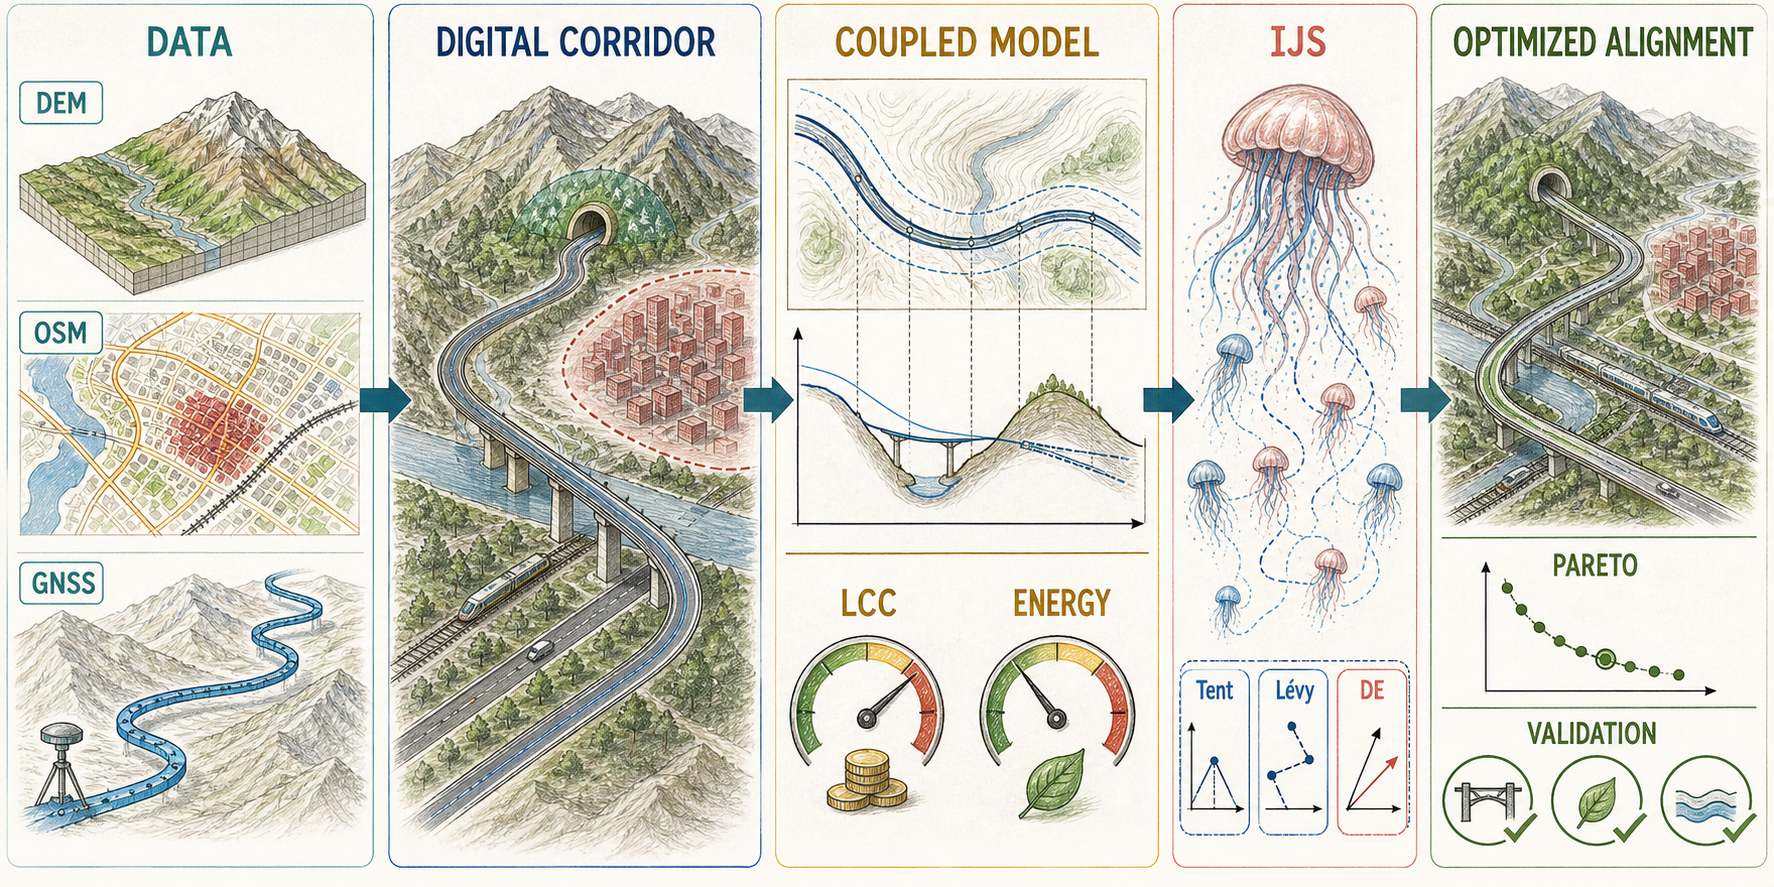
\includegraphics[width=\textwidth]{method_overview_handdrawn.png}
\caption{Data-driven workflow for collaborative three-dimensional highway alignment optimization. The hand-drawn scientific illustration highlights the information flow; the mathematical definitions are given in Sections~\ref{sec:model} and \ref{sec:solver}.}
\label{fig:overview}
\end{figure*}

\section{Related research}

\subsection{Three-dimensional alignment optimization}

Early simultaneous models demonstrated that horizontal and vertical decisions should not be optimized independently \cite{chew1989}. Evolutionary encoding subsequently made non-convex three-dimensional search practical \cite{jong2003}. GIS-based studies expanded the feasible region and allowed environmental layers to influence routing \cite{kang2012,davey2017}. Corridor-constrained horizontal search \cite{mondal2015} and rigorous vertical-alignment formulations \cite{akhmet2022} improved mathematical tractability, while bi-objective road and railway models incorporated cost, hazard and ecological impacts \cite{hirpa2016,zhang2020,song2022}.

Recent end-to-end models integrate BIM or intelligent path planners \cite{han2023,pu2024}. These methods improve automation but do not eliminate the need for transparent engineering accounting. In particular, a spatial intersection must lead to a structure or clearance decision, terrain sampling must follow the candidate line, and existing network connections must be preserved. This paper therefore prioritizes traceable geometry-to-cost mappings over an opaque surrogate objective.

\subsection{Life-cycle cost and traffic energy}

The underlying life-cycle model follows the categories in Lin \cite{lin2025}: land acquisition, bridges/tunnels, road works, maintenance and earthwork. Vehicle operation is relevant because geometric consistency affects emissions and energy demand \cite{llopis2019}. Electric-vehicle energy is especially sensitive to grade, mass, auxiliaries and regenerative behavior \cite{dimartino2022}. Rather than adding fuel and electricity in incompatible physical units, the present framework monetizes both over the analysis period. This does not claim that money is a complete environmental metric; it supplies a consistent decision scale while physical fuel and electricity components remain reportable.

\subsection{Optimization algorithms and objective decision}

NSGA-II remains a standard multi-objective benchmark \cite{deb2002}, but direct evolutionary search becomes expensive as the number of profile variables increases. Jellyfish Search models ocean-current and active/passive motion \cite{chou2021}. The present IJS adds three complementary mechanisms: a Tent map for initial coverage, L\'evy flights for non-local exploration and differential evolution (DE) for vector-wise refinement \cite{storn1997}. The mechanisms are not assumed beneficial a priori; Section~\ref{sec:ablation} measures their isolated and combined contributions.

Entropy weighting is based on the information concept of Shannon \cite{shannon1948}. Here it is applied only after feasibility and non-dominance screening. Thus a high weight cannot compensate for a geometric violation, and an infeasible solution cannot be selected merely because its cost is low.

\section{Data-driven mathematical formulation}\label{sec:model}

\subsection{Study corridor and data fusion}

The case is the Xunfengzhou--Huangcun portion of Guangzhou North Ring Expressway, a two-way six-lane urban expressway with a measured centerline length of 22.462 km. The input comprises 14,018 GNSS points with plan coordinates and elevations. These points define the existing scheme M-A, the fixed plan endpoints and the vertical tie-in elevations.

Terrain is sampled from AWS Terrain Tiles \cite{awsterrain}. Sixty zoom-level-14 tiles are decoded at approximately 8.8 m pixel spacing. Because the available surface represents the built road, a $\pm60$-m road mask is removed and interpolated from neighboring terrain to obtain a quasi-natural ground. Its correlation with the measured centerline elevation is 0.915 after a constant vertical-datum correction. This reconstruction is imperfect but applies the same terrain accounting to the existing and optimized alternatives.

OSM \cite{haklay2008,osmlicense} supplies roads, railways, watercourses and building footprints. After removing the North Ring Expressway and parallel facilities, the obstacle set contains 4,807 road features, 857 railway features and 338 river/canal features. Building footprints are rasterized on a 25-m grid and smoothed with a 200-m kernel. Thresholds are calibrated against the maximum density already traversed by M-A: Tier 2 is a hard exclusion, Tier 1 is passable with a soft discouragement, and Tier 0 is unrestricted. Figure~\ref{fig:case} shows the aligned layers.

\begin{figure*}[t]
\centering
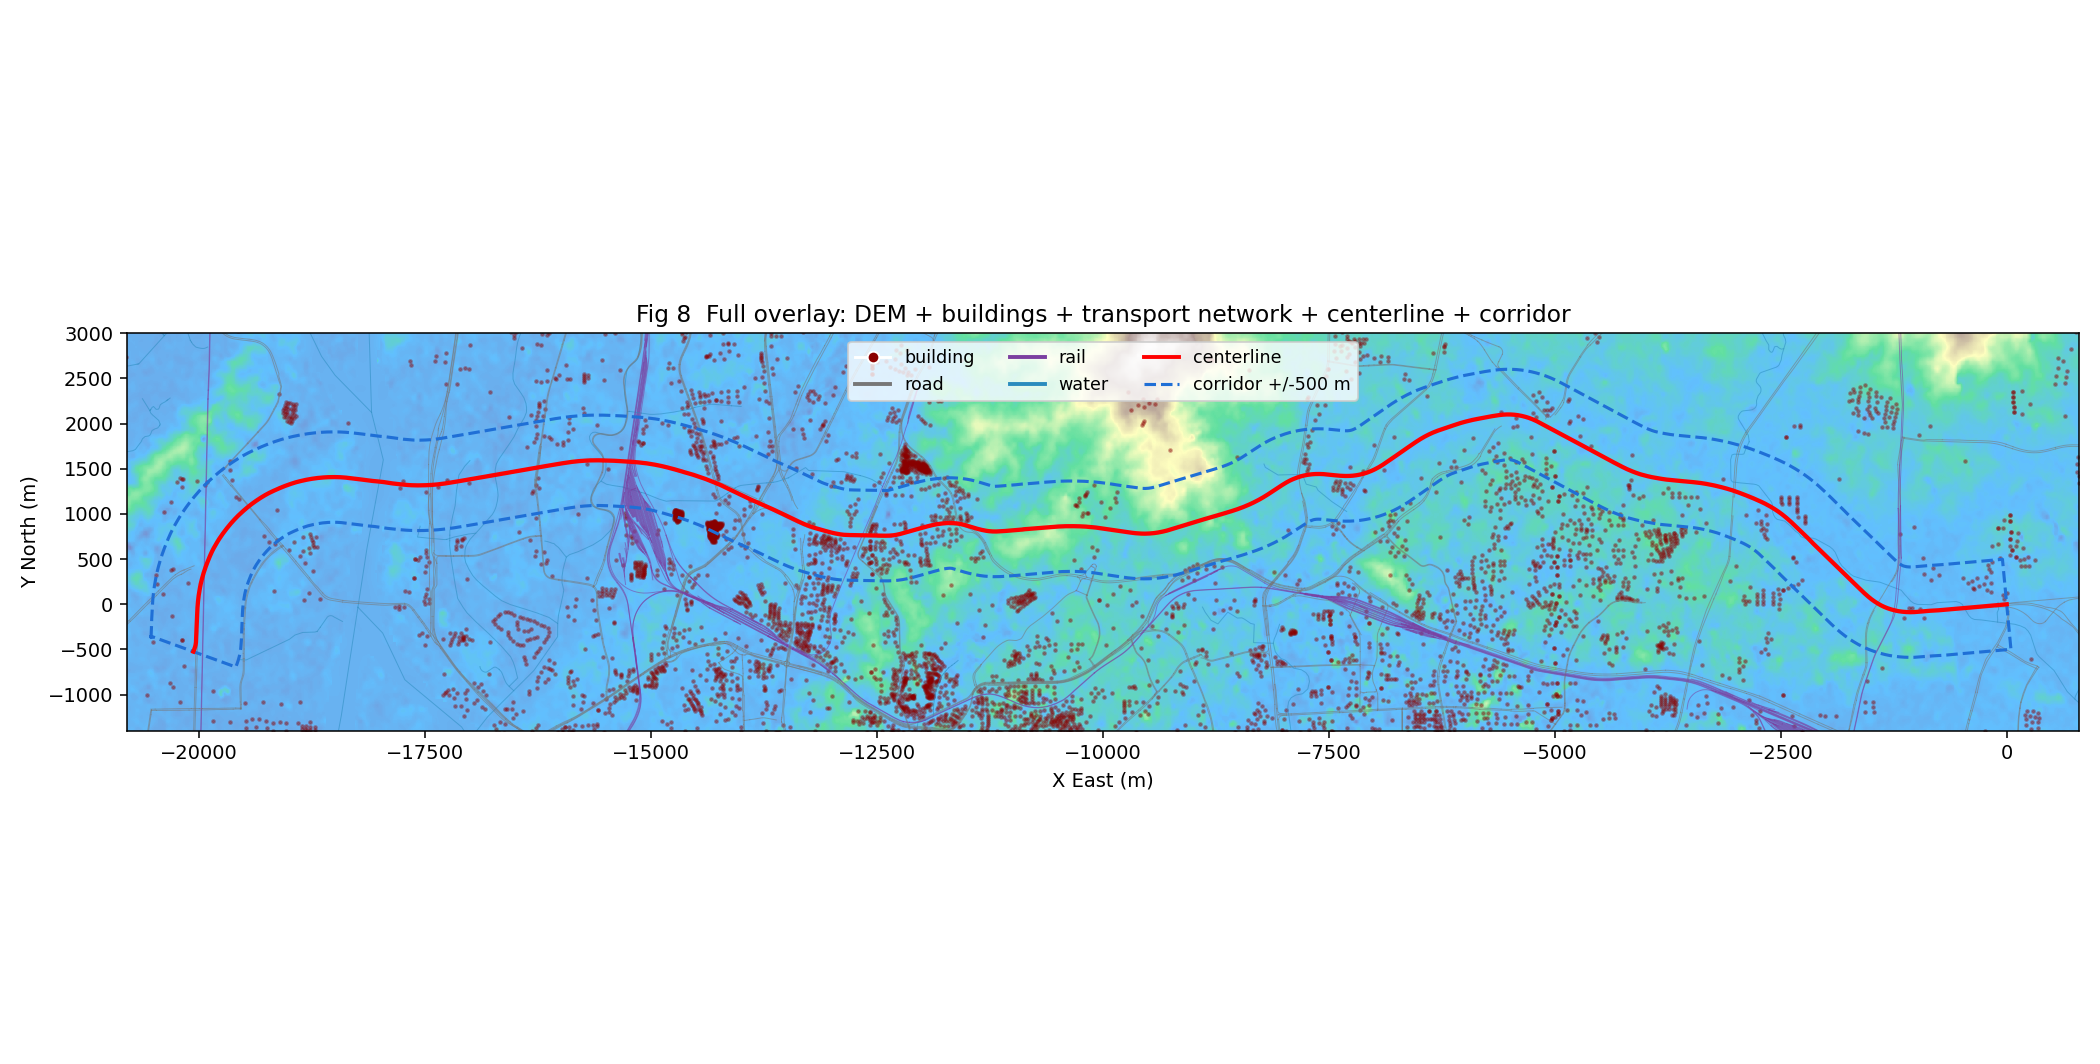
\includegraphics[width=\textwidth]{case_data_layers.png}
\caption{Case-study data layers in the local engineering coordinate system: DEM, OSM buildings, roads, railways, watercourses, measured centerline and the $\pm500$-m corridor. OSM completeness limitations are discussed in Section~\ref{sec:limitations}.}
\label{fig:case}
\end{figure*}

\subsection{Collaborative decision variables}

Let the measured plan line be $\bm r_0(s)=[x_0(s),y_0(s)]^\top$ with unit normal $\bm n(s)$, $s\in[0,L_0]$. A candidate plan is represented by a normal offset
\begin{equation}
\delta(s)=\sum_{k=1}^{50}a_k\sin\left(\frac{k\pi s}{L_0}\right), \qquad
|a_k|\leq \frac{W}{k^2},
\label{eq:sine}
\end{equation}
where $W=500$ m in the main experiment. The sine basis fixes both endpoints and attenuates high-frequency curvature. Offset control points are reconstructed by a cubic spline and evaluated on a 10-m grid.

The vertical profile uses $M=225$ stations (approximately 100 m apart). Normalized variables generate segment grades, but the start and end design elevations $z_0$ and $z_L$ are tied to the measured road. For raw grade perturbations $h_i\in[-1,1]$, segment lengths $\Delta s_i$ and maximum grade $g_{\max}=0.04$, define
\begin{align}
\bar h&=\frac{\sum_i h_i\Delta s_i}{\sum_i\Delta s_i},\qquad
g_{\mathrm{req}}=\frac{z_L-z_0}{\sum_i\Delta s_i},\\
g_i&=g_{\mathrm{req}}+\lambda g_{\max}(h_i-\bar h),
\label{eq:grades}
\end{align}
where $\lambda\in[0,1]$ is the largest scaling that retains $|g_i|\leq g_{\max}$. Consequently $\sum_i g_i\Delta s_i=z_L-z_0$ exactly. The current decision dimension is $50+225=275$; the roughly 150 plan reconstruction controls are not optimization dimensions.

\subsection{Life-cycle cost}

The first objective is
\begin{equation}
\min C=C_R+C_B+C_S+C_Q+C_{TU},
\label{eq:lcc}
\end{equation}
where $C_R$ is land acquisition, $C_B$ bridge/tunnel cost, $C_S$ basic subgrade and pavement cost, $C_Q$ discounted maintenance and $C_{TU}$ earthwork/haulage. Unit rates follow the source thesis and the 2025 Guangzhou governmental estimation guideline \cite{guangzhou2025}. The analysis period is 30 years with a 5\% discount rate.

At station $j$, let $h_j=z_j-z^g_j$ be the design-to-ground height, $B$ the formation width and $m$ the side-slope ratio. The approximate cross-sectional earthwork area is
\begin{equation}
A_j=B|h_j|+m h_j^2.
\end{equation}
Volumes are integrated by the average-end-area method. If fill/cut cost exceeds the corresponding bridge/tunnel cost, or if $|h_j|>30$ m, structural substitution is triggered. The selected structure cost replaces rather than supplements earthwork in that interval, preventing double counting and ``free floating road'' solutions.

For each candidate plan, intersections with OSM road classes primary and above, railways and watercourses trigger bridges. If $\theta_q$ is the crossing angle and $b_q$ the nominal obstacle width, the required crossing interval is
\begin{equation}
\ell_q=\frac{b_q}{\max(\sin\theta_q,\sin15^\circ)}+2E_{\mathrm{ext}},
\end{equation}
where $E_{\mathrm{ext}}=75$ m is the approach extension. Gaps under 100 m are merged. Ramp-function cost is calibrated from the seven existing interchanges and kept invariant, whereas mainline bridge length is geometric. A connected terrain region above 70 m, closed morphologically over 500 m, defines the Baiyun ecological mandatory-tunnel zone. Its area (19.2 km$^2$) and M-A crossing length (1.28 km) agree with independent project information (about 21 km$^2$ and 1.35 km, respectively).

\subsection{Mixed fuel--electric traffic energy}

The second objective monetizes lifetime operation of a mixed fleet:
\begin{equation}
\min E=\sum_{y=1}^{30}\frac{365\,Q_y}{(1+r)^y}
\left[(1-p_{EV})c_f e_f(\bm x)+p_{EV}c_e e_e(\bm x)\right],
\label{eq:energy}
\end{equation}
where $Q_y$ is AADT, $p_{EV}=0.30$, $c_f$ and $c_e$ are fuel and electricity prices, and $e_f,e_e$ are per-vehicle route consumption. The baseline uses AADT=30,000 vehicles/day, gasoline/electricity prices of 8 RMB/L and 0.8 RMB/kWh, and the same discount rate as cost.

For a fuel vehicle, the traction load includes aerodynamic, rolling, grade and residual lateral forces. With speed $v$, mass $m_v$, aerodynamic coefficient $C_d$, frontal area $A_f$, grade angle $\alpha$ and curve radius $R$, these are
\begin{align}
F_{air}&=\tfrac12\rho C_d A_fv^2, & F_r&=C_rm_vg\cos\alpha,\\
F_g&=m_vg\sin\alpha, &
F_a&=\max\left(0,\frac{m_vv^2/R-m_vgS_p}{N_vC_s}\right).
\end{align}
Internal and external power are converted to fuel flow following the calibrated model in Lin \cite{lin2025}. The printed $10^{-3}$ multiplier in the source expression for $F_a$ is omitted: retaining it makes lateral resistance roughly five orders too small and removes the plan-curvature energy channel. This dimensional correction is explicitly disclosed rather than silently absorbed into calibration.

Electric consumption uses the same longitudinal resistances, drivetrain efficiencies, regenerative sign handling and a 15-kWh/100-km auxiliary term. Fuel and electric use are retained separately before monetary aggregation. The current main experiment evaluates a representative travel direction; fixing both endpoint elevations removes the former net-downhill bookkeeping exploit. A bidirectional mean is identified as a required extension in Section~\ref{sec:limitations}.

\subsection{Constraints and decision rule}

The hard engineering set includes: fixed plan and profile endpoints; corridor width; $R(s)\geq400$ m for 100 km/h design speed; $|g_i|\leq4\%$; normalized adjacent grade change; crossing skew angle $\theta\geq15^\circ$; and zero Tier-2 penetration. Values follow JTG D20-2017 \cite{jtgd20} where directly applicable. Local violations use the sum of mean and maximum relative violation, so a short severe defect cannot disappear in a long route average.

For objectives $C$ and $E$, a common baseline population supplies reference scales $C_{ref}$ and $E_{ref}$. Entropy weights $w_C,w_E$ produce
\begin{equation}
F(\bm x)=w_C\frac{C(\bm x)}{C_{ref}}+w_E\frac{E(\bm x)}{E_{ref}}
+P(\bm x)+0.22\frac{L_{T1}(\bm x)}{L(\bm x)}.
\label{eq:scalar}
\end{equation}
IJS is run over a weight sweep. The final decision is selected by four gates: hard feasibility, budget $C\leq1.1C_{M-A}$, non-dominance, and entropy-weighted compromise within the surviving front.

\section{Improved Jellyfish Search}\label{sec:solver}

\subsection{Mechanisms}

The original JS alternates an ocean-current update toward the best solution with active/passive movement within the population \cite{chou2021}. The IJS implementation adds:

\begin{itemize}[leftmargin=*]
\item \textbf{Independent Tent initialization.} Each individual uses an independent chaotic chain with $\mu=1.99$. The exact value $\mu=2$ is avoided because finite-precision binary arithmetic collapses to zero; a single shared chain is avoided because it creates correlated individuals.
\item \textbf{Domain-scaled L\'evy flight.} The heavy-tailed perturbation is scaled by $0.01(\bm u-\bm l)$. The former unscaled implementation had only a 0.48\% acceptance rate because a unit step is not meaningful across heterogeneous variable ranges.
\item \textbf{DE refinement.} Mutation and crossover with $CR=0.5$ form a trial vector from population differences, followed by elitist acceptance \cite{storn1997}.
\end{itemize}

Each IJS generation therefore has about three population-equivalent evaluation phases; this is reported rather than comparing equal generation counts as equal effort. A two-phase penalty schedule uses 0.3 of the nominal penalty in the first half and 3.0 in the second half, allowing exploration near feasibility boundaries before final constraint recovery. Figure~\ref{fig:flow} gives the full process.

\begin{figure}[t]
\centering
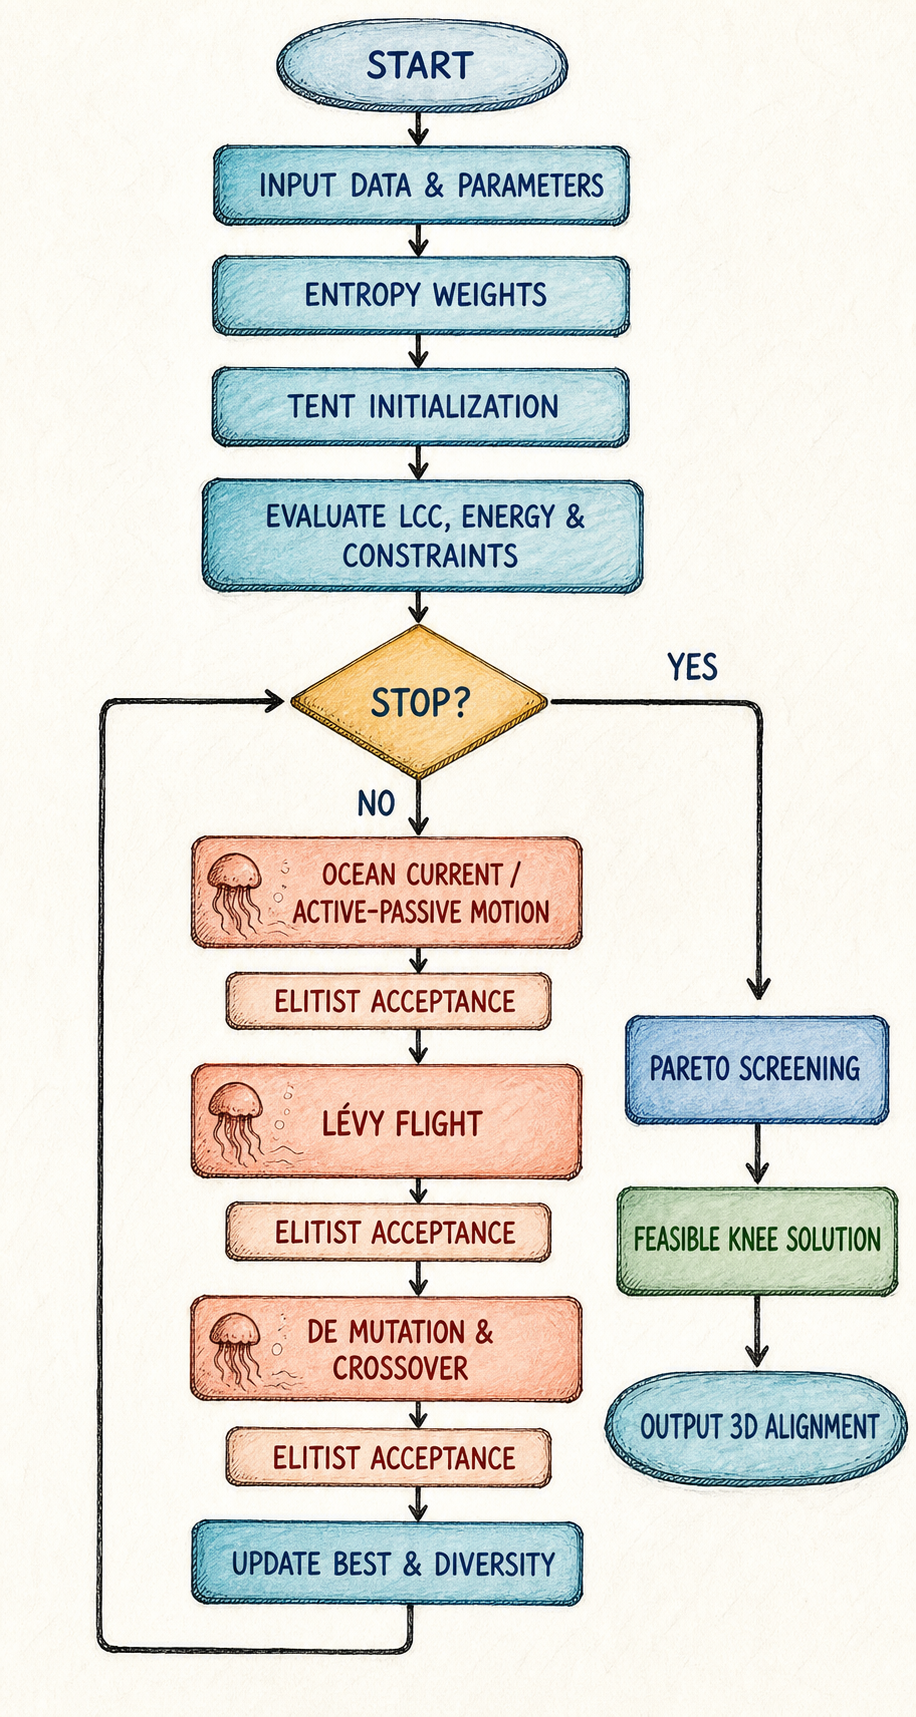
\includegraphics[height=.72\textheight,keepaspectratio]{ijs_flowchart_handdrawn.png}
\caption{IJS solution and decision flow. Each operator is followed by elitist acceptance; the stopping branch proceeds to feasibility and Pareto screening.}
\label{fig:flow}
\end{figure}

\subsection{Experimental protocol}

The scheme experiment uses population 200, 1,000 IJS iterations and 21 Pareto weights (a later visual sweep uses 40). Objectives are evaluated at approximately 10-m spacing. The baseline, cost-only and joint alternatives use the same data and reference scales.

The ablation fixes the measured plan and solves the 225-dimensional profile problem. Five reported variants (JS, +Tent, +L\'evy, +DE and complete IJS) are selected from the full $2^3$ design. Each has 30 independent runs, population 200 and 500 iterations. The multi-algorithm experiment compares IJS, JS, NSGA-II, real-coded GA, PSO and GWO on six joint scales, with profile spacing 500, 400, 300, 200, 100 and 50 m (95--500 dimensions). Each algorithm--scale pair has 10 seeds. Wilcoxon rank-sum and Friedman rank tests \cite{wilcoxon1945,friedman1937} are applied to final objectives. Sensitivity analysis re-optimizes every sampled scenario rather than merely re-evaluating a fixed alignment.

\section{Results}

\subsection{Current engineering scheme}

Table~\ref{tab:current} and Figure~\ref{fig:scheme} report the current main result: $\pm500$ m, density constraints active and endpoint elevations anchored. M-C reduces $C$ by 8.33\% and $E$ by 3.00\%. The route is 12 m longer (+0.05\%), demonstrating that the saving is not an artificial consequence of a shorter path. Bridge/tunnel cost decreases by 237 million RMB, while earthwork rises by 15 million RMB. The net effect is physically interpretable: the optimizer accepts more earthwork and a slightly longer route to reduce structural exposure and operating energy.

\begin{table}[t]
\centering
\caption{Current endpoint-anchored, density-constrained result.}
\label{tab:current}
\begin{threeparttable}
\begin{tabular}{lrrr}
\toprule
Metric & M-A existing & M-C optimized & Change \\
\midrule
Life-cycle cost ($10^8$ RMB) & 26.4061 & 24.2078 & $-8.33\%$ \\
Traffic energy ($10^8$ RMB) & 13.9460 & 13.5278 & $-3.00\%$ \\
Length (km) & 22.4618 & 22.4741 & $+0.05\%$ \\
Minimum radius (m) & 422 & 421 & feasible \\
Slope-hazard index & 3.309 & 3.298 & $-0.35\%$ \\
Tier-1 exposure (km) & $\approx2.00$ & 1.591 & $-20.5\%$ \\
Tier-2 exposure (km) & 0 & 0 & feasible \\
Penalty & 0 & 0 & feasible \\
\bottomrule
\end{tabular}
\begin{tablenotes}\footnotesize
\item Cost and energy are 30-year discounted monetary quantities. Tier-1 is passable with a soft term; Tier-2 is forbidden.
\end{tablenotes}
\end{threeparttable}
\end{table}

\begin{figure*}[t]
\centering
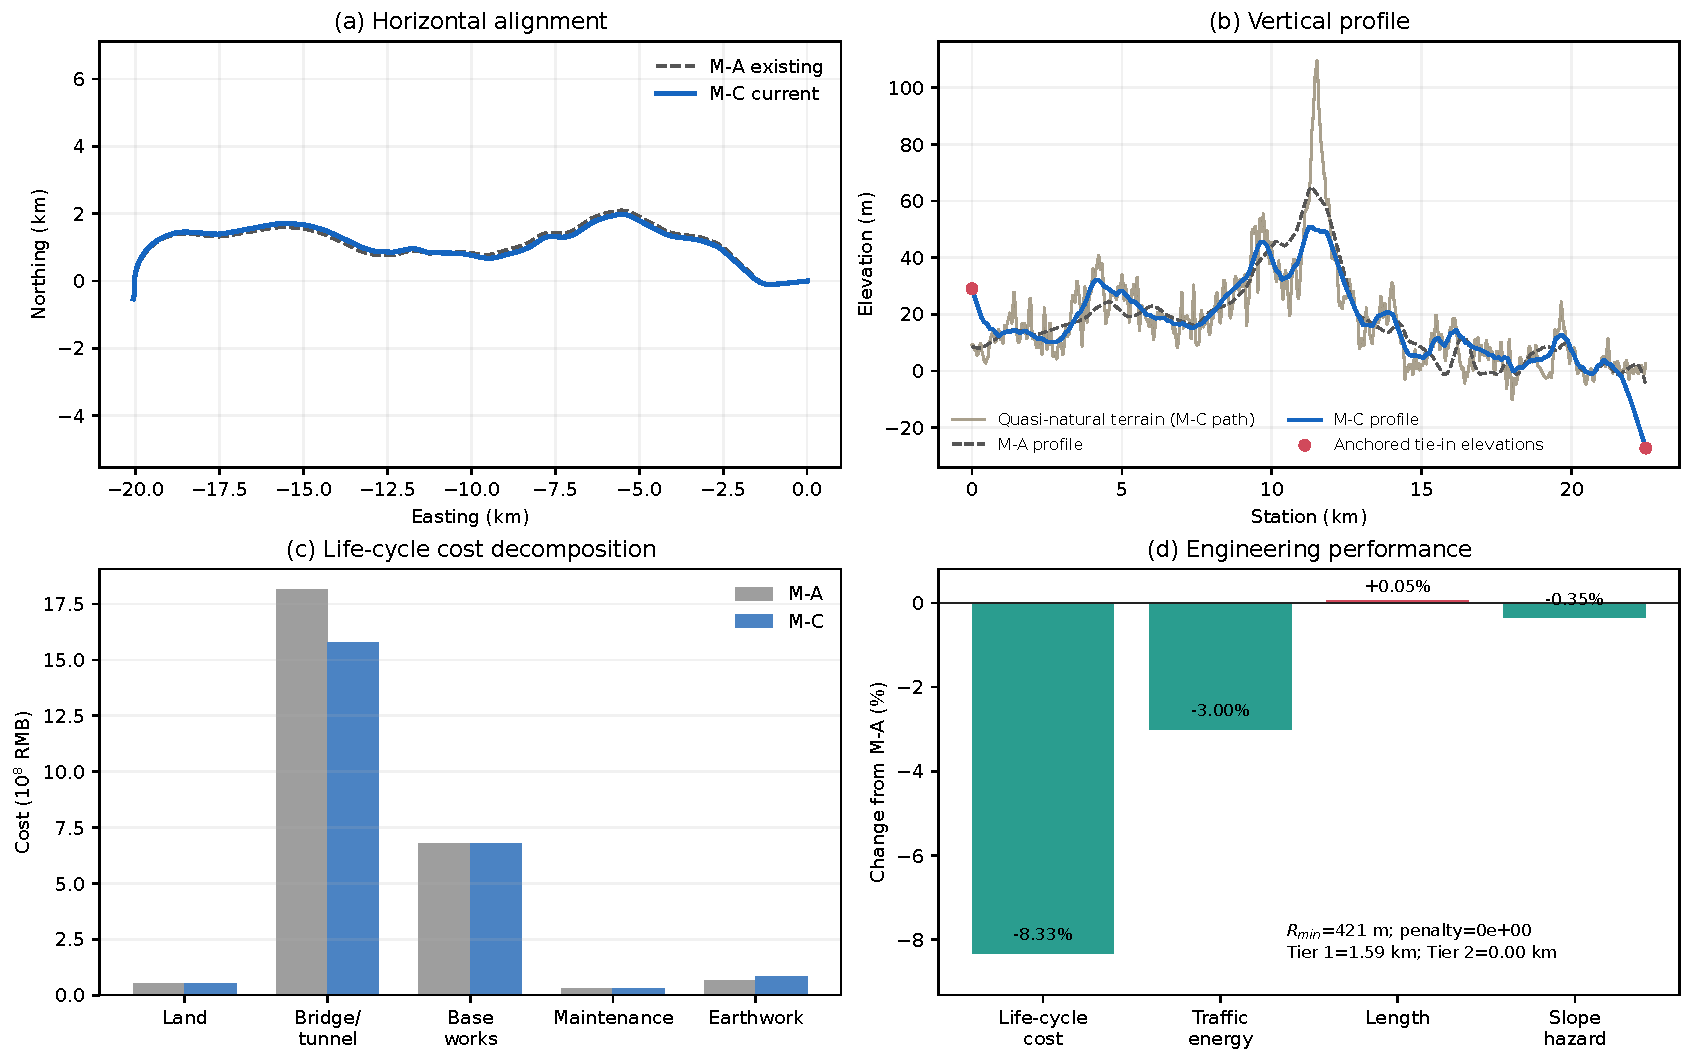
\includegraphics[width=\textwidth]{current_scheme_summary.pdf}
\caption{Current M-A/M-C comparison: (a) plan, (b) endpoint-anchored profile, (c) life-cycle cost decomposition and (d) headline changes. The increased earthwork and small length increase are shown explicitly.}
\label{fig:scheme}
\end{figure*}

The selected line crosses 1.591 km of Tier 1 and no Tier 2. Figure~\ref{fig:density} verifies this against the density field. It also avoids treating the existing route as an exception: Tier thresholds are calibrated so that a density already traversed by M-A is evidence of passability, while denser connected cores remain forbidden.

\begin{figure*}[t]
\centering
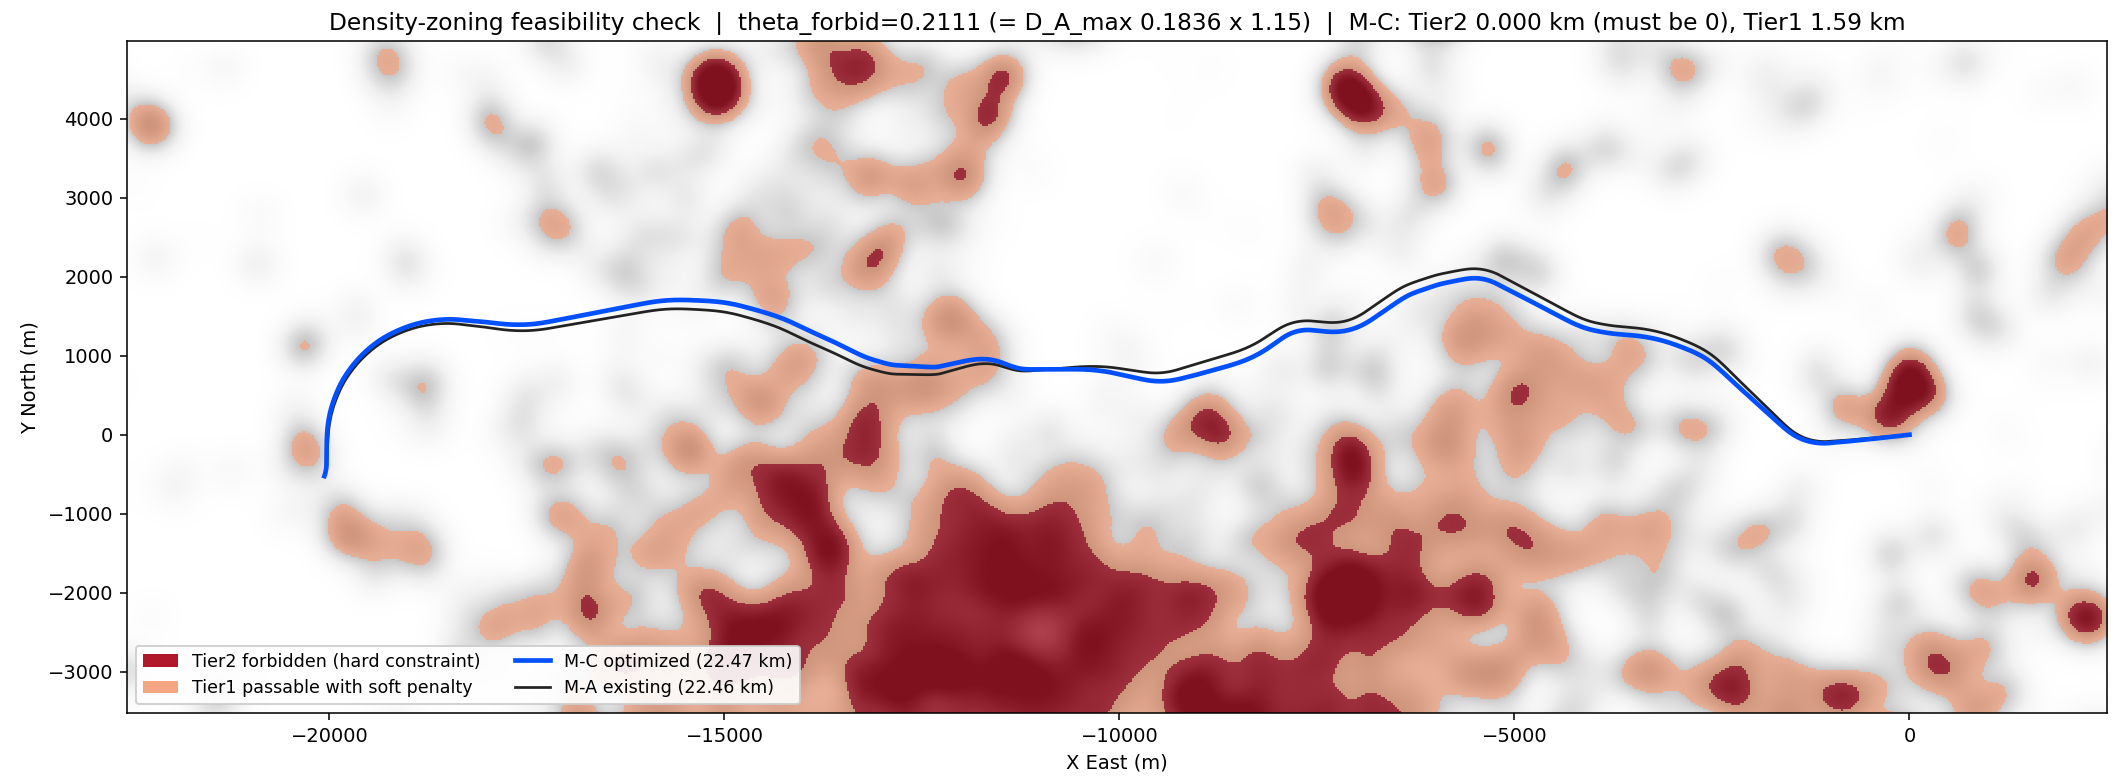
\includegraphics[width=\textwidth]{density_feasibility_w500.png}
\caption{Building-density feasibility check. The current M-C line avoids Tier-2 cores and reduces Tier-1 exposure to 1.59 km.}
\label{fig:density}
\end{figure*}

The current Pareto set (Figure~\ref{fig:pareto}) contains costly structure-heavy energy endpoints as well as the practically relevant cluster. Feasibility and the 10\% budget gate remove those extremes before entropy selection. The chosen M-C is therefore a constrained compromise, not simply the minimum of a globally normalized weighted sum.

\begin{figure}[t]
\centering
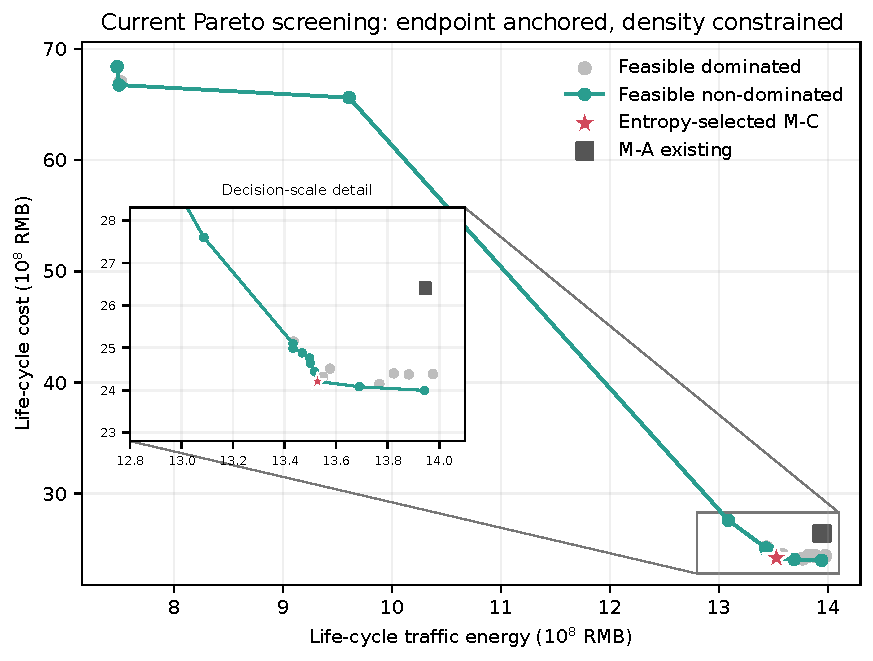
\includegraphics[width=\linewidth]{current_pareto_density.pdf}
\caption{Feasible and non-dominated screening under the current endpoint and density constraints.}
\label{fig:pareto}
\end{figure}

Figure~\ref{fig:3d} provides the spatial interpretation. The present M-C contains approximately 4.08 km of OSM-triggered crossing bridges and 0.75 km in the Baiyun ecological tunnel zone. These values differ from earlier repository figures because the current density-constrained solution is used here.

\begin{figure*}[t]
\centering
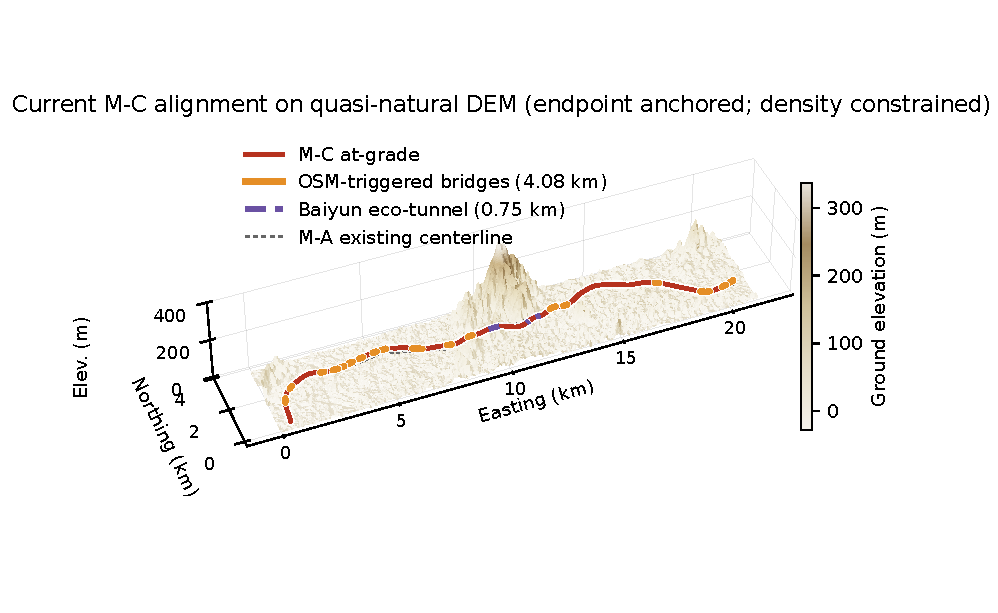
\includegraphics[width=\textwidth]{current_alignment_3d.pdf}
\caption{Current M-C on the quasi-natural DEM. At-grade, OSM-triggered bridge and ecological-tunnel intervals are distinguished; M-A is shown as a dashed reference.}
\label{fig:3d}
\end{figure*}

\subsection{Why collaborative optimization is necessary}

A controlled experiment completed immediately before adding the density tiers used identical objective references and equal evaluation budgets for joint and two-stage methods. The existing line had $C=26.4061$, $E=13.9460$. The two-stage method obtained $C=23.1582$ and $E=13.4569$, apparently better than the joint result ($C=24.2239$, $E=13.4766$). However, its minimum radius was 397 m and penalty $7.36\times10^{-2}$, whereas the joint solution had 401 m and zero penalty. The lower two-stage objectives are therefore not admissible evidence of superiority. Freezing the plan after stage one removed the degrees of freedom needed to reconcile crossing-bridge positions and the vertical profile near the curvature boundary. This result supports collaborative optimization through constraint coupling rather than through selective objective reporting.

\subsection{IJS mechanism ablation}\label{sec:ablation}

Table~\ref{tab:ablation} shows the 30-run ablation. IJS reduces mean $F$ from 0.9133 to 0.6808 (25.45\%) and reaches the final JS level in 187 generations rather than 500. DE produces the dominant isolated gain (24.17\%, $p=3.02\times10^{-11}$). L\'evy gives a smaller 3.79\% improvement ($p=0.0555$), while Tent improves 1.58\% but is not significant alone ($p=0.464$). Thus the evidence supports ``DE-dominant, L\'evy-assisted, Tent-diversified'' rather than attributing all improvement to chaotic initialization.

\begin{table}[t]
\centering
\caption{Thirty-run IJS ablation on the 225-dimensional profile problem.}
\label{tab:ablation}
\begin{tabular}{lrrrrr}
\toprule
Variant & Mean $F$ & SD & $F_{100}$ & Gain vs JS & $p$ \\
\midrule
JS & 0.9133 & 0.0637 & 2.547 & -- & -- \\
JS+Tent & 0.8989 & 0.0605 & 2.227 & 1.58\% & 0.464 \\
JS+L\'evy & 0.8787 & 0.0558 & 2.095 & 3.79\% & 0.0555 \\
JS+DE & 0.6926 & 0.0315 & 1.679 & 24.17\% & $3.02\times10^{-11}$ \\
IJS & \textbf{0.6808} & 0.0340 & \textbf{1.292} & \textbf{25.45\%} & $3.02\times10^{-11}$ \\
\bottomrule
\end{tabular}
\end{table}

\begin{figure*}[t]
\centering
\begin{subfigure}{.48\textwidth}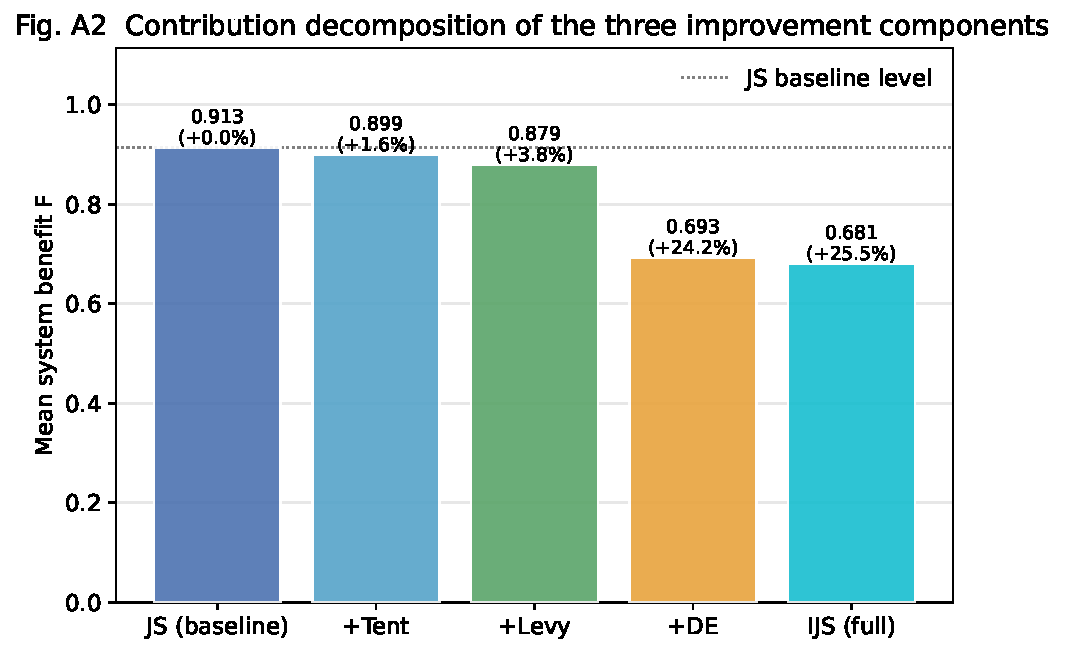
\includegraphics[width=\linewidth]{ablation_contributions.pdf}\caption{Component contribution.}\end{subfigure}\hfill
\begin{subfigure}{.48\textwidth}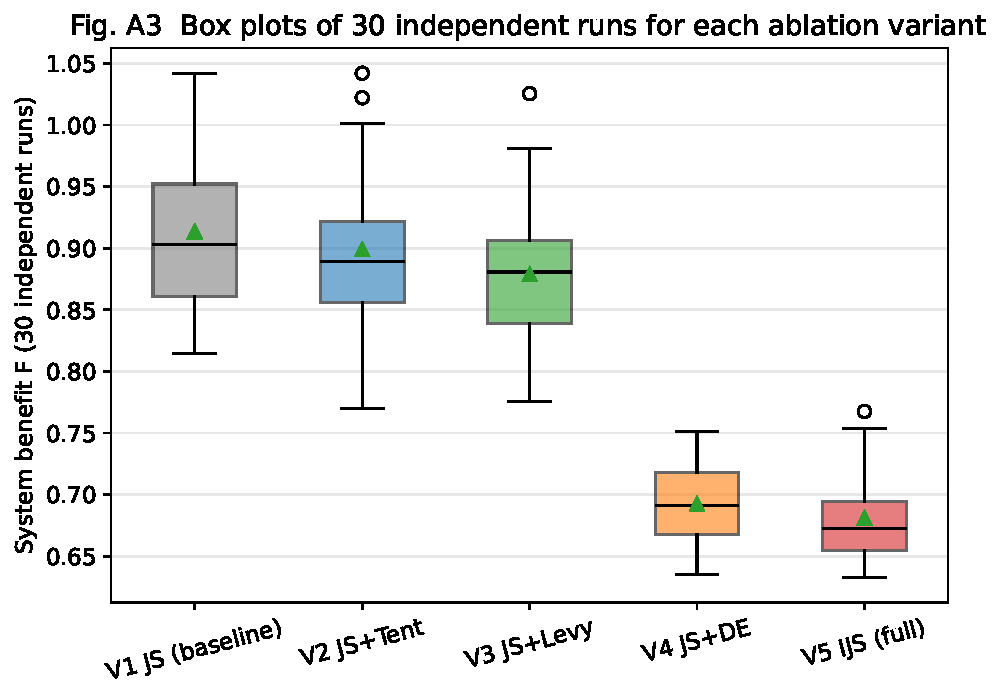
\includegraphics[width=\linewidth]{ablation_boxplot.pdf}\caption{Run-to-run distribution.}\end{subfigure}
\caption{Ablation results. Lower $F$ is better.}
\label{fig:ablation}
\end{figure*}

Mechanism instrumentation clarifies the result. Independent Tent chains replace 132 of 200 random initial individuals. DE still contributes about 0.018 improvement in the final 100 generations, indicating local refinement rather than only early acceleration. A pre-defined ``escape after 20 stagnant generations'' statistic is not applicable because complete IJS rarely experiences a 20-generation stagnant interval; reporting it as zero would incorrectly imply failure.

\subsection{Algorithm benchmark}

IJS achieves the lowest best-of-10 $F$ at all six joint scales (Table~\ref{tab:benchmark}). Friedman average rank is 1.0, and pairwise Wilcoxon tests against all competitors are below $8.8\times10^{-4}$. At PJ6 (500 dimensions), IJS and JS retain 10/10 feasibility, while GWO has 0/10 and the other methods suffer large penalty-dominated objectives. The result is stronger than a low-dimensional curve-fitting comparison because scale changes only profile resolution; the engineering model remains fixed.

\begin{table*}[t]
\centering
\caption{Best objective among ten runs across joint problem scales. Lower is better.}
\label{tab:benchmark}
\begin{tabular}{lrrrrrr}
\toprule
Algorithm & PJ1 (95) & PJ2 & PJ3 & PJ4 & PJ5 & PJ6 (500) \\
\midrule
IJS & \textbf{0.6570} & \textbf{0.5928} & \textbf{0.7054} & \textbf{0.7053} & \textbf{0.7682} & \textbf{0.8305} \\
JS & 0.6697 & 0.5977 & 0.7127 & 0.7108 & 0.7911 & 0.8465 \\
NSGA-II & 0.6737 & 0.6095 & 0.7203 & 0.7161 & 0.7939 & 12.0355 \\
GA & 0.6939 & 0.6269 & 0.7322 & 0.7370 & 4.5169 & 23.4880 \\
PSO & 0.6841 & 0.6184 & 0.7324 & 0.7527 & 7.7130 & 31.8988 \\
GWO & 0.6715 & 0.6111 & 0.7161 & 0.7149 & 1.0843 & 1.3556 \\
\bottomrule
\end{tabular}
\end{table*}

\begin{figure*}[t]
\centering
\begin{subfigure}{.64\textwidth}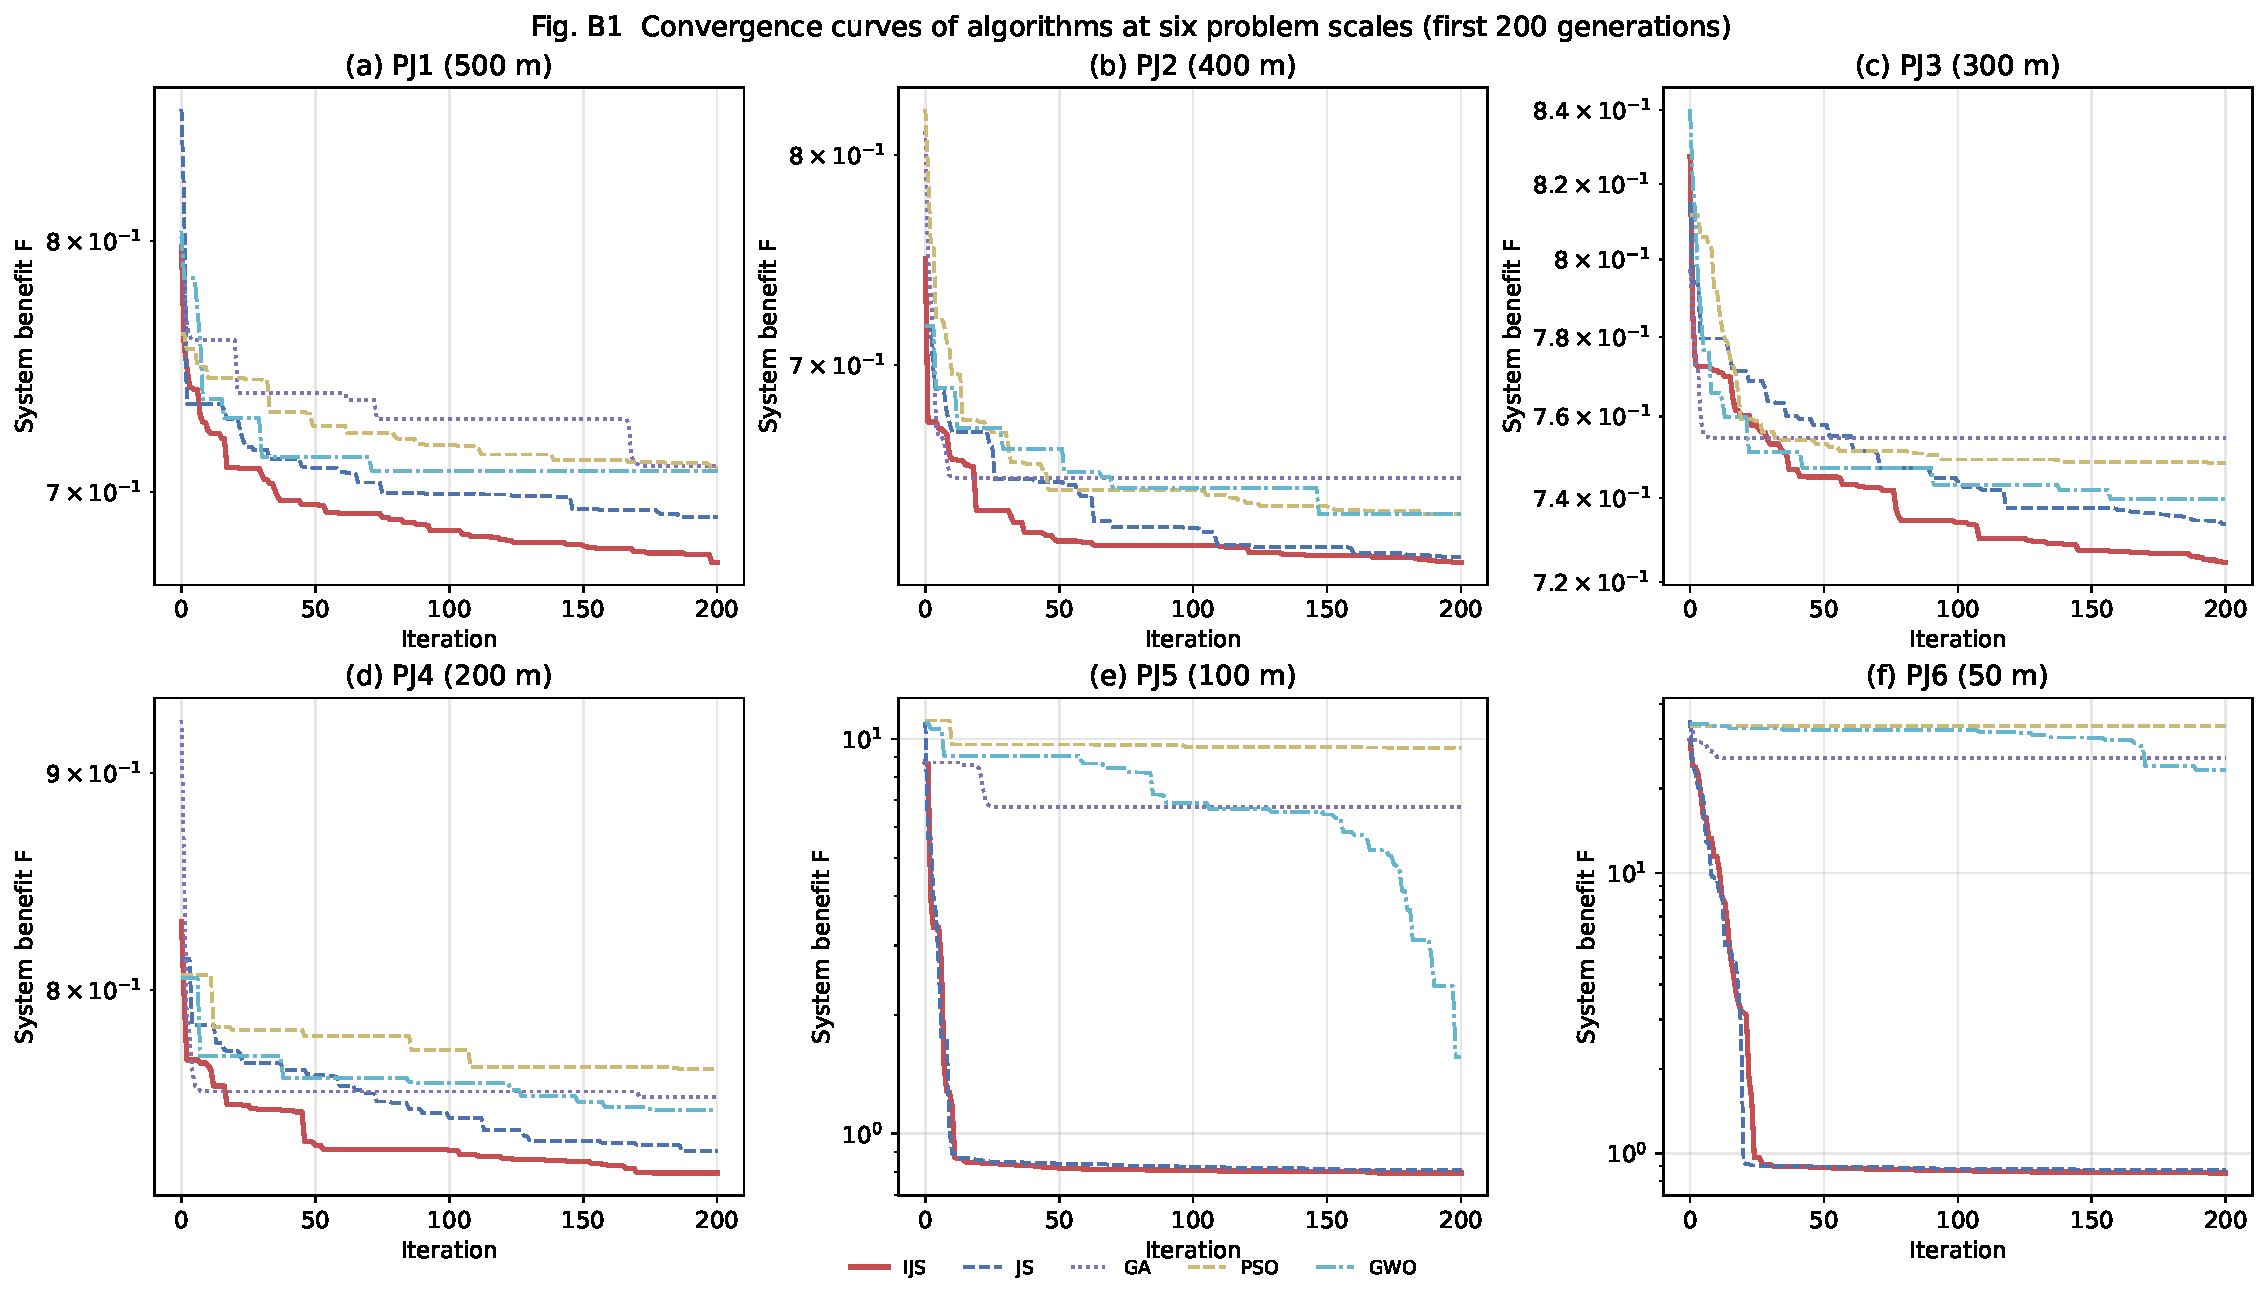
\includegraphics[width=\linewidth]{algorithm_convergence.pdf}\caption{Convergence over six scales.}\end{subfigure}\hfill
\begin{subfigure}{.33\textwidth}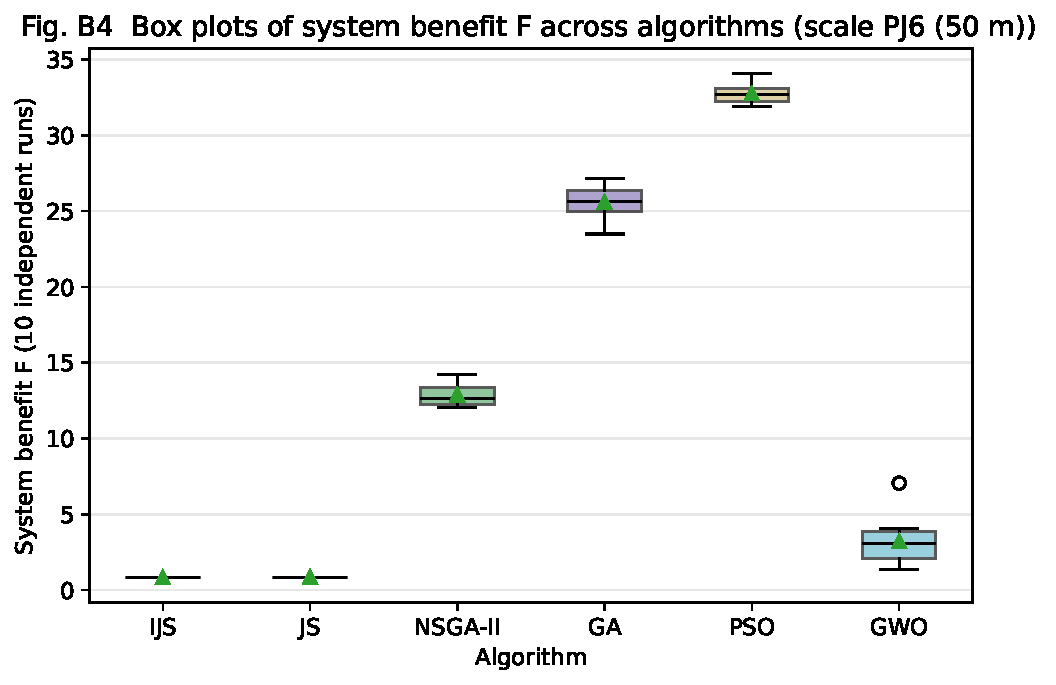
\includegraphics[width=\linewidth]{algorithm_pj6_boxplot.pdf}\caption{PJ6 distribution.}\end{subfigure}
\caption{Multi-algorithm benchmark. IJS uses roughly three population-equivalent evaluations per generation; runtime and NFE are therefore reported with quality.}
\label{fig:benchmark}
\end{figure*}

IJS takes about twice the wall time of one-phase competitors at PJ1--PJ5 because L\'evy and DE add evaluations. Its advantage is optimization quality and feasibility under a declared evaluation multiplier, not nominal speed per iteration. Future comparisons should equalize NFE as well as seeds; the present tables expose the multiplier to prevent an unfair generation-only claim.

\subsection{Re-optimization sensitivity}

All 237 sensitivity points converge to feasible solutions. Traffic growth dominates the energy response; cost is comparatively robust to demand, fleet and price factors because infrastructure cost is incurred largely at construction. Raising EV penetration moderates the high-growth energy burden, while simultaneous fuel and electricity price growth increases the monetized energy objective.

Corridor width produces a strong then saturating cost response: in the matched re-optimization experiment, $C$ decreases from 2.568 billion RMB at 200 m to 2.239 billion RMB at 2,500 m. The benefit accelerates once the line can leave the ecological-tunnel zone, then becomes limited by urban and geometric constraints. Varying bridge approach extension $E_{ext}$ from 50/75/100 m shifts $C$ to 2.281/2.355/2.474 billion RMB, whereas $E$ remains near 1.355 billion RMB. This separates an uncertain structural-cost convention from the principal energy conclusion.

\begin{figure*}[t]
\centering
\begin{subfigure}{.48\textwidth}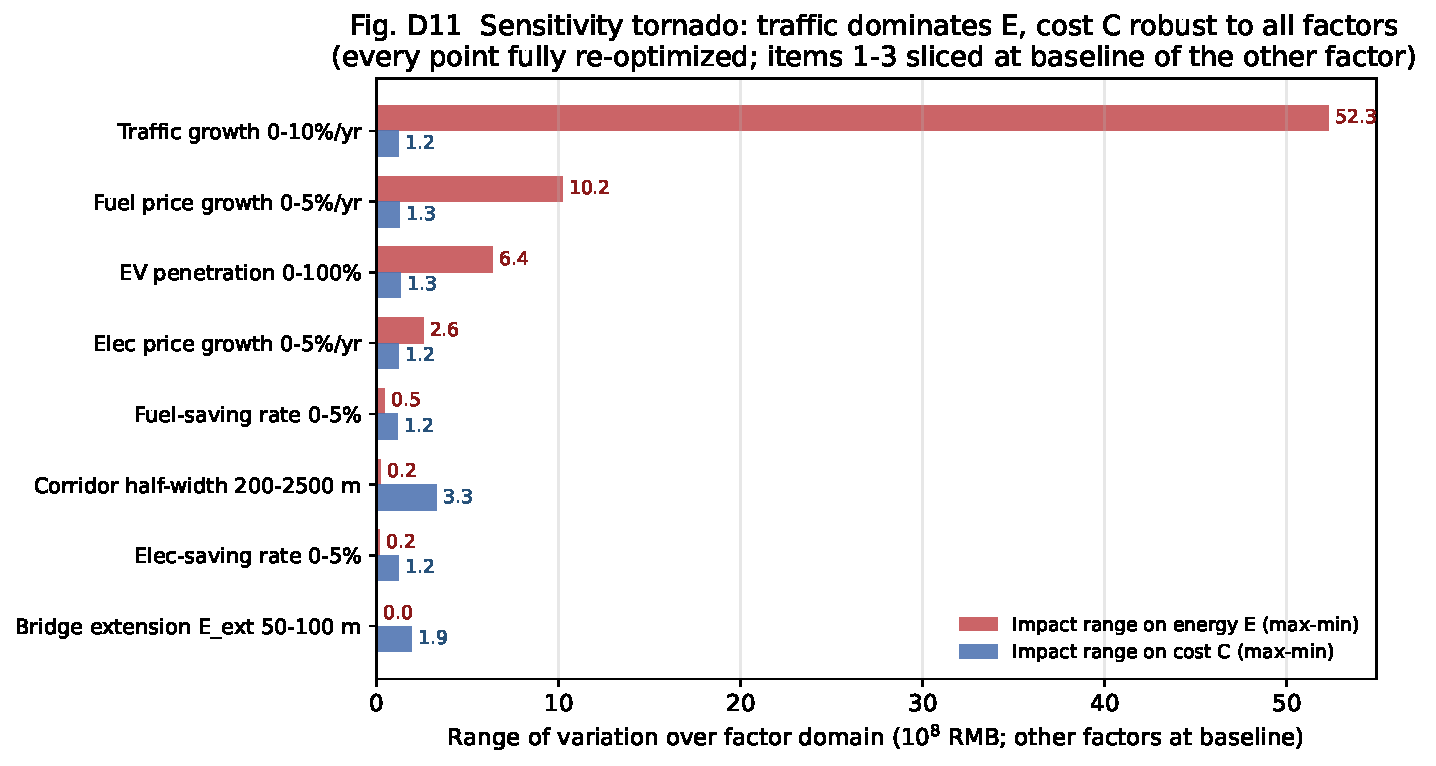
\includegraphics[width=\linewidth]{sensitivity_tornado.pdf}\caption{Relative importance of scenario factors.}\end{subfigure}\hfill
\begin{subfigure}{.48\textwidth}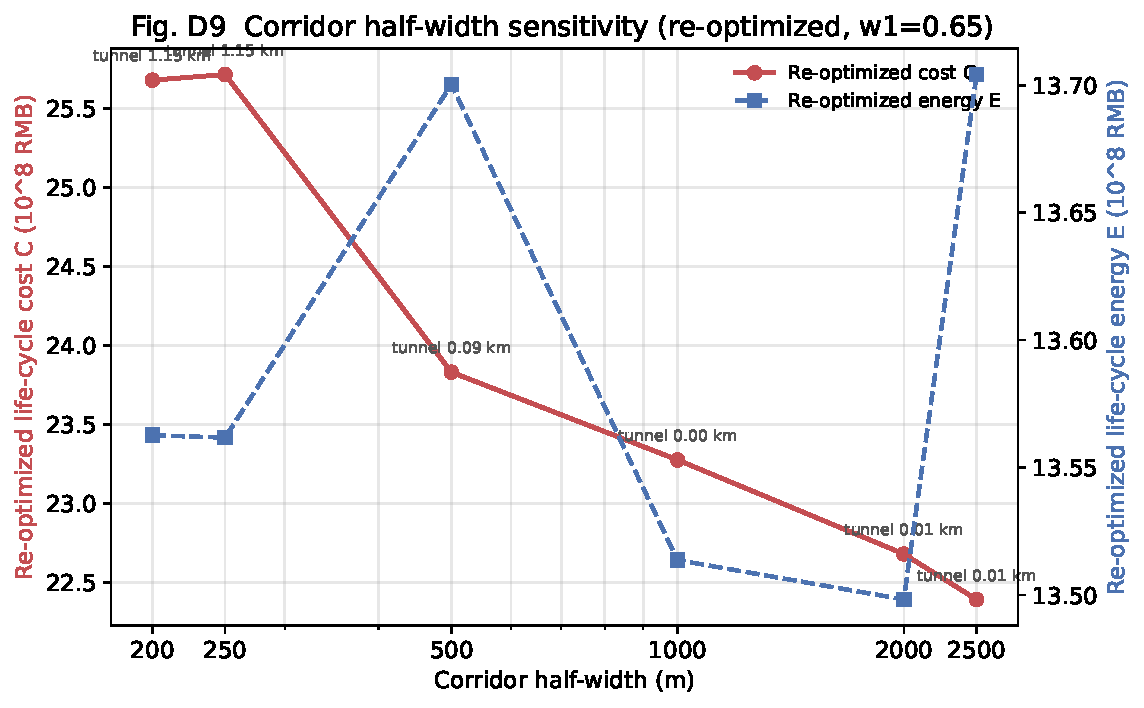
\includegraphics[width=\linewidth]{corridor_sensitivity.pdf}\caption{Corridor-width re-optimization.}\end{subfigure}
\caption{Sensitivity results. Every plotted point is re-optimized rather than evaluated on a frozen line.}
\label{fig:sensitivity}
\end{figure*}

\section{Discussion}

\subsection{Engineering meaning of the improvement}

The 8.33\% cost decrease should not be interpreted as a generic saving for all expressways. It is a case-specific comparison under common data and prices. Its importance lies in the mechanism. M-C is slightly longer and has higher earthwork than M-A, but it reduces structural cost and energy while remaining outside Tier 2. The optimizer is therefore trading physical components, not merely exploiting route length. The endpoint constraints further prevent a candidate profile from receiving an unearned energy benefit by starting high and ending low.

The pre-density two-stage control illustrates why objective values alone are insufficient. Its lower $C$ and $E$ result from a line with $R_{min}=397$ m. Once feasibility is enforced, the claimed advantage disappears. Collaborative search preserves the ability to relocate horizontal crossings while reshaping the profile, which is particularly relevant where an OSM-triggered bridge and a grade transition interact.

\subsection{Role of DEM and OSM}

DEM changes the objective landscape because the ground is sampled under every candidate plan. Without it, lateral motion would affect only length and abstract land price. OSM makes structural demand and urban exposure geometry-dependent. The approach is not a substitute for survey-grade design: the dataset lacks bridge-deck elevations, parcel acquisition costs and complete building attributes. Its value is to move early-stage optimization from a one-dimensional centerline profile toward a reproducible spatial screening model.

The building tiers also clarify a policy distinction. Tier 2 is an exclusion because its density exceeds what the existing expressway demonstrates as traversable. Tier 1 is not forbidden; it carries a soft discouragement. This avoids the unrealistic claim that an urban expressway can never pass developed land while still steering alternatives away from dense clusters. In practice the soft term should be replaced by parcel-level acquisition and resettlement data.

\subsection{Algorithmic interpretation}

The ablation does not support a simplistic ``chaos improves everything'' narrative. Tent initialization alone is small and statistically non-significant. DE explains most of the quality gain, while L\'evy contributes moderate exploration and Tent improves initial coverage after numerical correction. Their combination matters because the feasible region is narrow and multi-modal: initialization supplies coverage, L\'evy supplies non-local moves and DE refines coupled plan/profile vectors.

The benchmark further shows that feasibility is a primary algorithmic outcome. At high resolution, several competitors return penalty-dominated solutions even when their unconstrained search appears active. IJS's higher evaluation cost is justified only when this feasibility and quality gain matters. Surrogate models, parallel evaluation or decomposition are promising routes to reduce cost.

\subsection{Limitations and validity threats}\label{sec:limitations}

The following limitations are material rather than cosmetic.

\begin{enumerate}[leftmargin=*,label=(\arabic*)]
\item The quasi-natural DEM is reconstructed by removing the present road influence, not observed before-construction terrain. Its 8.8-m pixel spacing cannot resolve local drainage and retaining structures.
\item OSM coverage is heterogeneous. Secondary roads do not trigger bridges, and bridge vertical clearance is not constrained because obstacle deck elevations are unavailable. A 15-degree skew limit is calibrated against the existing minimum of 15.6 degrees.
\item The Tier-1 weight (0.22 in normalized $F$) is a policy discouragement, not a measured demolition bill. The density constraint has been applied only to the latest scheme experiment; the earlier ablation and benchmark use the common pre-density objective and are identified as algorithmic evidence rather than direct current-scheme replications.
\item The energy objective is monetary and evaluates a representative travel direction. Endpoint anchoring removes net-elevation arbitrage, but a two-direction traffic-weighted model with calibrated regenerative braking is needed for final design.
\item Adjacent grade change is a proxy for vertical-curve smoothness. Explicit crest/sag curve lengths, non-overlap, sight distance, clothoid/arc segmentation and complete horizontal--vertical coordination checks are not yet implemented.
\item Cost rates represent early-stage estimates. Geological investigation, hydrology, parcel ownership, construction staging, embodied carbon and uncertainty are outside the current model.
\item The selected current scheme is a single optimization outcome. Algorithm statistics are strong in the dedicated experiments, but the density-constrained scheme itself requires a multi-seed replication before a final submission claim of stochastic robustness.
\end{enumerate}

These limitations define the boundary of the claim: the framework supports reproducible corridor-level decision and method comparison; it does not replace detailed geometric or construction design.

\section{Conclusions}

This study presents a data-driven, collaborative horizontal--vertical highway alignment framework that connects three-dimensional geometry to life-cycle cost and mixed fuel--electric traffic energy. The model extends an earlier mathematical base with quasi-natural DEM sampling, OSM-triggered bridges, an ecological tunnel zone, building-density tiers, structural substitution and exact endpoint tie-ins. IJS supplies a corrected and empirically tested search process, while feasibility and non-dominance precede entropy-based decision.

For Guangzhou North Ring Expressway, the current $\pm500$-m density-constrained result reduces cost by 8.33\% and monetized energy by 3.00\%, with $R_{min}=421$ m, zero hard penalty and no Tier-2 penetration. The line is slightly longer and uses more earthwork, so the improvement is attributable to a transparent structural/operational trade rather than length alone. A two-stage control shows that superficially better objectives can be infeasible. Ablation and six-scale benchmarking identify DE as the principal IJS improvement and show consistent IJS superiority, while 237 re-optimized scenarios support qualitative robustness.

The next research stage should implement bidirectional energy, survey-grade obstacle elevations, explicit vertical curves and sight distance, parcel/embodied-carbon objectives, uncertainty-aware costs and multi-seed replication of the latest density-constrained scheme. These additions would move the framework from auditable corridor planning toward design-grade decision support.

\section*{Data and code availability}
The manuscript is generated from the RoadPlan experiment repository. GNSS and project-derived files may be subject to owner restrictions; processed DEM/OSM layers, source code, fixed random seeds, result JSON files and figure-generation scripts are organized for reproducibility. A public archive and DOI should be inserted after anonymization review: \nolinkurl{[DATA-REPOSITORY-DOI-PLACEHOLDER]}.

\section*{CRediT authorship contribution statement}
\textbf{[Author name placeholders]}: Conceptualization, Methodology, Software, Validation, Investigation, Data curation, Visualization, Writing---original draft, Writing---review \& editing. Contributions must be replaced with the actual author roles before submission.

\section*{Declaration of competing interest}
The authors declare that they have no known competing financial interests or personal relationships that could have appeared to influence the work reported in this paper. This statement must be confirmed by all authors before submission.

\section*{Acknowledgements}
Funding agency, grant number and non-author contributions are intentionally anonymized and must be completed before submission.

\bibliographystyle{elsarticle-num}
\bibliography{../references}

\end{document}
